\subsection{Invariant preservation}
\label{sec:properties:inv}
As presented in the RedBlue consistency chapter (Chapter~\ref{chapter:redblue}), the methodology
for identifying restrictions imposed on RedBlue orders for maintaining invariants is to check if
a shadow operation is invariant safe or not. If not, to avoid invariant 
violations, the generation and replication of all non-invariant safe shadow operations must be coordinated. 
However, we observed that for some non-invariant safe shadow operations $u$, the corresponding violation
only happens when a particular subset of non-invariant safe shadow operations are not partially ordered. 
To eliminate all invariant violating executions with a minimal amount of coordination, therefore, 
we need to precisely define, for each violation, the minimal
set of non-invariant safe shadow operations that are involved. We call this
set an {\tt invariant-conflict operation set}, or short, {\tt I-conflict set}. We formally define this 
as follows.

\if 0
\begin{mydef}
[Invariant safe condition] Given a shadow operation $h_{u}(S)$, its invariant safe
condition is a function $isc(S')$ of all valid state $S'$ and $S$ such that $isc(S')$ holds iff
$S' + h_{u}(S)$ is also a valid state. 
\label{def:isafecond}
\end{mydef}

For simplicity, for any shadow operation $u$, we denote $u.isc$ as its invariant preserving condition. Apparently,
if $u$ is an invariant safe shadow operation, then $u.isc = $ {\tt true} w.r.t all valid state.
\fi
\changebars{
\begin{mydef}
[Invariant-conflict operation set] A set of
shadow operations $G$ is an invariant-conflict operation set (or short, I-conflict set), if
the following conditions are met:
\begin{itemize}
 \item $\forall u \in G$, $u$ is non-invariant safe;
 \item $|G| > 1$;
 \item $\forall u \in G$, $\forall$ sequence P consisting of all shadow operations in G except u, i.e.,
$P = (G \setminus \{u\}, <)$, and $\exists$ a reachable and valid state $S$, s.t. $S(P)$ is valid, and
$S(P + u)$ is invalid.
\end{itemize}
\label{def:iconflictset}
\end{mydef}
}{}

In the above definition, the last point asserts that
$G$ is minimal, i.e., removing one shadow operation from it will no
longer lead to invariant violations. We will use the following example to illustrate
the importance of minimality. Imagine that we have an auction on an item $i$ 
being replicated across three sites such as US, UK and DE,
and having initially a $5$ dollar bid from $Charlie$. Suppose also that three shadow operations,
namely, $placeBid'(i, Bob, 10)$, $placeBid'(i, Alice, 15)$, and 
$closeAuction'(i)$ are accepted concurrently at the three locations, respectively. 
After applying all of them against the same initial state at every site,
we end up with an invalid state, where $Charlie$ rather than $Bob$ and $Alice$ won
the auction. This invariant violating execution
involves three concurrent shadow operations, but one of the two bid placing shadow
operations is not necessarily to be included in $G$, as even after excluding
the request from either $Bob$ or $Alice$, the violation still remains. \changebars{According
to Definition~\ref{def:iconflictset}, $\{ placeBid', closeAuction'\}$ is an \texttt{I-conflict set},
while $\{placeBid', placeBid', closeAuction'\}$ is not. Intuitively, avoiding invariant
violations is to prevent all operations from the corresponding \texttt{I-conflict} set
from running in a coordination-free manner. The minimality property enforced in the \texttt{I-conflict set}
definition allows us to avoid adding unnecessary restrictions.}{}  

Based on the above definition, we then can
 formulate the invariant preservation property into the following theorem.

\if 0
\begin{figure*}[t!]
\begin{minipage}[t]{0.5\textwidth}
\subfloat[R-Order $O$ of an execution $E$, which violates invariants]{\label{fig:invarexamplerorder}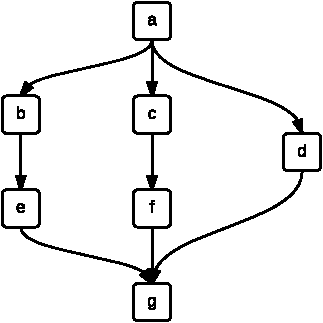
\includegraphics[width=0.8\textwidth]{./por/figures/por_invariant_preserving_chart_rorder.pdf}}
\end{minipage}
\begin{minipage}[t]{0.5\textwidth}
\centering
\subfloat[Shortest linear prefix of $O$ observing invalid state]{\label{fig:invarexamplerprefix}
\includegraphics[width=1.0\textwidth]{./por/figures/por_invariant_preserving_chart_P.pdf}}\\
\subfloat[R-Order $O'$ of $P$]{\label{fig:invarexampleshortestrorder}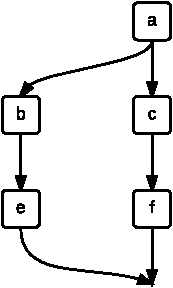
\includegraphics[width=0.3\textwidth]{./por/figures/por_invariant_preserving_chart_shortest_rorder.pdf}}\\
\subfloat[A permutation of $P$, where $T = f+e$ is the suffix]{\label{fig:invarexamplerpermu}
\includegraphics[width=1.0\textwidth]{./por/figures/por_invariant_preserving_chart_permu.pdf}}
\end{minipage}
\caption{Illustrative example for the proof of the invariant preservation theorem~\ref{theorem:invpreserve}. Rectangle boxes represent
shadow operations. The set $\{e, f\}$ is I-conflict set, while $\{b, c\}$ is not. $d$ is invariant safe.}
\label{fig:invarexample}
\end{figure*}
\fi

\begin{theorem}
{\bf Invariant preservation theorem:} Given a \PRCAJ\ system $\mathscr{S}$
with a set of restrictions
$R_{\mathscr{S}}$, for any execution of $\mathscr{S}$ that starts from a valid state, no site
is ever in an invalid state, if the following conditions are met:
\begin{itemize}
 \item for any its {\tt I-conflict} set $G$, there exists
a restriction $r(u, v)$ in $R_{\mathscr{S}}$, for at least one pair of shadow operations $u, v \in G$; and
 \item for any pair of shadow operations $u$ and $v$, $r(u, v)$ in  $R_{\mathscr{S}}$ if $u$ and $v$ don't commute.
\end{itemize}

\label{theorem:invpreserve}
\end{theorem}
\if 0
To prove the above theorem, we need to introduce the following lemma, which states that
in a legal serialization, for any shadow operation $h_u(S)$, let $S'$ be the state before
executing $h_u(S)$, if $S \neq S'$, then there must exist at least a shadow operation $v$ such that
$u$ and $v$ are not ordered w.r.t the corresponding R-Order, i.e., $u$ and $v$ are running concurrently.

\begin{lemma}\label{lem:concurrentexists}
Let $O_i=(U,<_i)$ be  a legal serialization of R-Order $O=(U,\prec)$, 
where $\forall m, n\in U, m\not\prec n \wedge n\not\prec m \implies $ $m$ and $n$
commute. Let $S_0$ be the initial state, for any
shadow operation $h_u(S) \in U$, let $S'$ be the state obtained by sequentially applying all shadow
operations in $U$ that precede $h_u(S)$ according to $<_i$ against $S_0$.
If $S \neq S'$, then $\exists v\in U$ such that $h_u(S)\not\prec v$ and $v\not\prec h_u(S)$.
\end{lemma}

\noindent{\bf Proof:}
We assume by contradiction that $S \neq S'$ but $\not\exists v\in U$ such that $h_u(S)\not\prec v$ and $v\not\prec h_u(S)$. This implies
that $\forall v \in U$, if $v \neq h_u(S)$, then $v \prec h_u(S)$ or $h_u(S) \prec v$. It then follows from \PRCN\ (Def~\ref{def:porconsistency})
and the legal serialization definition (Def~\ref{def:legalserial}) that for any legal serialization $L$ of $O$, $h_u(S)$ partitions
$L$ into two sequences $P$ and $Q$, where $P$ is a sequence containing exactly all shadow operations preceding $h_u(S)$ according to $\prec$ 
and $Q$ is a sequence containing exactly all shadow operations following $v$ according to $\prec$. 
Let $L_{c}$ the causal serialization of $O$ from site $i$, which is the primary site of the generator operation $g_u$ of $h_u(S)$. 
Let $L_c = P_c + h_u(S) + Q_c$. It follows from the definition of causal legal serialization (Def ~\ref{def:causalserial}) that $S_0(P_c) = S$.
Let $L_1$ and $L_2$ be two legal serializations of $O$ such that $L_1 = P_1 + h_u(S) + Q_1$ and $L_2 = P_2 + h_u(S) + Q_2$. 
It then follows from Lemma~\ref{lem:canSwap}, ~\ref{lem:adjexists}, ~\ref{lem:adjacentconvergent}
and the assertion that any pair of concurrent shadow operations in $O$ commute that $S_0(P_1) = S_0(P_2) = S_0(P_c)$. 
As a result, in every legal serialization including $L_c$, $S' = S$. Contradiction is found.
 \qed
\fi

%With the above lemma, we can prove the invariant preservation theorem as follows:
We prove the invariant preserving theorem by contradiction as follows:
\changebars{
\noindent{\bf Proof:} 
We assume by contradiction that
invariant violations are possible with a sufficient set of restrictions
$R_{\mathscr{S}}$ in place. Let $E$ be an invariant violating execution of $\mathscr{S}$ 
and let $O(U, \prec)$ be the R-Order of $E$. Let $O'(U_P, \prec)$
be a smallest R-Order that triggers the violation. $U_P \subset U$. Let $P(U_P,<)$ be a legal
serialization of R-Order $O'$. As $P$ violates the corresponding invariant, $S_{0}(P)$ is invalid. If $U_P$ is empty,
then $S_{0}(P) = S_0$, and $P$ is in a valid state. This violates the assumption
that $P$ is in an invalid state. The theorem is proved.

Then we consider that $U_P$ is non-empty. Let $G$ be the set of shadow operations
that are maximal according to $O'(U_P, \prec)$, i.e., $G \subset U_P$,
and $u \in G \Leftrightarrow \not\exists v \in U_P $ s.t. $u \prec v$.
The fact $U_P$ is not empty implies that $G$ is not empty as well. 

We first consider the case that $G$ contains invariant-safe shadow operations. Let $v$
be such an invariant safe shadow operation in $G$. If $v$ is not the last operation in $P$,
then it follows from Lemma~\ref{lem:canSwap}, ~\ref{lem:adjexists} and
the assertion that any pair of shadow operations that are not ordered in $\prec$ commute
w.r.t each other that we can swap $v$ and any shadow operation $u$, s.t. $u \in G$, $u \neq v$ and $v < u$.
This swapping process allows us to produce a new legal serialization $Q$ of the R-Order $O'$, where
$v$ appears as the last operation, i.e., $Q = Q' + v$. It also follows
from Lemma~\ref{lem:poradjacentconvergent} that $S_0(Q) = S_0(P)$. As $S_0(P)$ is invalid and $S_0(Q') + v = S_0(Q)$, 
$S_0(Q') + v$ is invalid. It then follows from the fact $v$ is invariant safe and the
invariant safe shadow operation definition (Def~\ref{def:isafeop}) that the state before applying $v$ must be invalid,
i.e., $S_0(Q')$ is not valid. This implies that there exists a smaller R-Order
$O''(U_P\setminus\{v\}, \prec)$ than $O'(U_P, \prec)$ that triggers the corresponding invariant. 
It contradicts with our assumption that $O'$ is a smallest R-Order observing invalid state.
Therefore, we only need to analyze the case when all shadow operations in $G$ are non-invariant safe.

We continue by checking if $|G| = 1$, i.e., $G$ contains a single non-invariant safe shadow operation. Let $v$ be that operation.
Let $L$ be the causal legal serialization of $O'$ from site $i$, where the generator of $v$ was executed.
Since $v$ is the only maximal element in $O'$, $L = L' + v$. It also follows from Lemma~\ref{lem:canSwap}, ~\ref{lem:adjexists},
Lemma~\ref{lem:poradjacentconvergent} and the assertion that any pair of unordered shadow operations commute that
$S_0(P) = S_0(L' + v)$, and as such $S_0(L' + v)$ is also invalid. It then follows from the correct shadow operation definition (Def~\ref{def:correctshadow})
that $S_0(L')$ is invalid. By similar logic as above, there exists
a smaller invariant violating R-Order than $O'$, and contradiction is found. As a result, $|G| > 1$.
 
Finally, we can further assume that $G$ is not an {\tt I-conflict} set.
Let $P'(U_P\setminus G, <)$ be the prefix of $P$, and $T(G, <)$ be the suffix of $P$ (i.e.,
$P = P' + T$). Let $S$ be $S_0(P')$. Let $u$ be the last shadow operation in $T$, i.e., $T = T' + u$.
It also follows from Lemma~\ref{lem:canSwap}, ~\ref{lem:adjexists},
Lemma~\ref{lem:poradjacentconvergent} and the assertion that any pair of unordered shadow operations commute that
we can construct all possible variants of $T'$ and all these sequences reach the same final state.
 Since $P's$ R-Order $O'$ is a smallest R-Order violating the corresponding invariant,
$S$ and $S(T')$ are valid, and $S(T)$ is invalid. Furthermore, it follows from the {\tt I-conflict set} 
definition (Def~\ref{def:iconflictset}) that $G$ is an {\tt I-conflict} set. It then follows from the assertion that 
for any {\tt I-conflict} set, there exists a restriction defined
over one pair of shadow operations in the set so that it is impossible to have all shadow operations in $G$
to not be ordered w.r.t each other in the R-Order $O'$. Therefore, $G$ cannot be a maximal element set of the R-Order $O'$. Contradiction is found.
\qed
}{}

\begin{algorithm}[th!]
\caption{State convergence restrictions discovery}
\label{alg:scdiscover}
\begin{algorithmic}[1]
\Function{scrdiscover}{$T$}\Comment{$T$: the set of shadow operations of the target system}
\State $R \leftarrow \{ \}$ \Comment{$R$: the restriction set}
\For{$i \leftarrow 0$ \texttt{to} $|T|-1$}
 \For{$j \leftarrow i$ \texttt{to} $|T|-1$}
    \If{$T_i$ \texttt{do not commute with} $T_j$}
     \State $R \leftarrow R \cup \{r(T_i, T_j)\}$
    \EndIf
 \EndFor
\EndFor

\Return $R$
\EndFunction
\end{algorithmic}
\end{algorithm}

\subsection{Identifying restrictions}
\label{ch:por:sect:identify}
As discussed in the previous subsection, the key to making a replicated system
adopt \PRCN\ and strike a right balance between performance and consistency semantics
is to identify a finest set of restrictions, which ensure both state convergence
and invariant preservation. With regard to the former property, we design a state convergence
restrictions discovery method (Algorithm~\ref{alg:scdiscover}), which
performs an operation commutativity analysis between pairs of operations. If
two operations do not commute, then a restriction between them is added to the returning
result restriction set.

\begin{algorithm}[th!]
\caption{I-conflict set discovery}
\label{alg:iconflictassess}
\begin{algorithmic}[1]
\Function{icsetdiscover}{$T$, $\wp(T)$}
\Comment{$T$: the set of operations of the target
system, $\wp(T)$ is the power set of $T$}

\If{$T.processed == $ {\tt true} or $|T| == 0$ }

  \Return
\EndIf

\State $result \leftarrow $ {\tt false} \Comment{{\tt true} indicates that
a subset of $T$ is {\tt I-conflict set}.}
\For{$j \leftarrow 2$ \texttt{to} $|T| - 1$}
\State let $\wp(T)_{j}$ be a subset of $\wp(T)$ s.t. each element in $\wp(T)_{j}$ has $j$ operations.
 \ForAll{$T' \in \wp(T)_{j}$}
    \Call{icsetdiscover}{$T'$, $\wp(T')$}
    \State $result \leftarrow result | T'.isIConflict$
 \EndFor
\EndFor

\If{$result == $ {\tt false}} \Comment{No subsets of $T$ are {\tt I-conflict set}, so we need to check $T$.}
 \If{$|T| == 1$} \Comment{Check self-conflicting}
   \If{$\neg(T_0.post \implies T_0.wpre)$} \Comment{$T_0$ is the 0-th element in $T$.}
     \State $T.isIConflict \leftarrow$ {\tt true}
   \EndIf
 \ElsIf{$|T| > 1$}
   \For{$i \leftarrow 0$ \texttt{to} $|T| - 1$} \Comment{$T_i$ is the $i$-th element in $T$.}
     \State $post \leftarrow \wedge _{x \in T\setminus{\{T_i\}}} x.post$
     \If{$\neg(post \implies T_i.wpre)$}
        \State $T.isIConflict \leftarrow$ {\tt true}
        \State break
     \EndIf
   \EndFor
 \EndIf
\EndIf
\State $T.processed \leftarrow$ {\tt true}
\EndFunction
\end{algorithmic}
\end{algorithm}

For discovering the required restrictions for invariant preservation, we have
to exhaustively explore all {\tt I-conflict} sets that trigger violations. However,
it is very challenging to achieve this since there might exists infinite number of
violating executions containing at least one I-conflict sets. Therefore, the exploration may not guarantee to terminate.
To solve this problem, we decide to take a more efficient approach,
in which we collapse many similar executions of a replicated system into a single
execution class. To do so, we use programming language techniques such as
weakest precondition and postcondition analysis. For every operation $u$, we denote
$u.wpre$ as its weakest precondition, which is a condition on
the initial state and the parameter values ensuring that $u$
always preserves invariants. We also denote $u.post$ as the postcondition summarizing
the final state after the execution of $u$ against all possible valid state. Algorithm~\ref{alg:iconflictassess}
is the algorithm we use to discover all {\tt I-conflict} sets for a target system. This algorithm
flags a set of operations $T$ as {\tt I-conflict} if either of the following two conditions is met:
a) $T$ contains a single operation $t$ and $t$ is self-conflicting, i.e., $t.wpre$ is
invalidated by $t.post$; and b) $|T| > 1$, any subset of $T$ is not {\tt I-conflict} (but
can be self-conflicting) and there exists an operation $u$ from $T$ such that $u.wpre$
can be invalidated by the compound postcondition of operations in $T\setminus \{u\}$.

\begin{algorithm}[t]
\caption{Invariant preservation restrictions discovery}
\label{alg:isdiscover}
\begin{algorithmic}[1]
\Function{iprdiscover}{$T$, $R$}\Comment{$T$: the set of shadow operations of the target
system, $R$: the restriction set}

\State \Call{icsetdiscover}{$T$, $\wp(T)$}\Comment{Compute all {\tt I-conflict sets}}

\ForAll{$T' \in \wp(T)$}
\If{$T'.isIConflict ==${\tt true}}
  \If{$|T'| == 1$}
     \State $R \leftarrow R \cup \{r(T'_0, T'_0)\}$ \Comment{Restrict self-conflicting operations}
  \ElsIf{$\forall u, v \in T', r(u, v) \not\in R$} \Comment{This set has not been restricted yet.}
     \State $R \leftarrow R \cup \{r(T'_i, T'_j)\}$, \texttt{where} $i \neq j$ and $T'_i, T'_j \in T'$\Comment{Restrict any pair of operations in $T'$}
  \EndIf
\EndIf
\EndFor

\Return $R$
\EndFunction
\end{algorithmic}
\end{algorithm}

Algorithm~\ref{alg:isdiscover} iterates all identified {\tt I-conflict} sets, and,
for each {\tt I-conflict} set $T$, it adds a restriction between any pair of operations from $T$
if no pairs of operations from that set is restricted. Otherwise, $T$ will be skipped.
This is because the relevant violating executions, where all shadow operations from $T$
are not restricted, have been already eliminated, and hence
there is no need to analyze $T$.

\begin{algorithm}[t]
\caption{Restriction set discovery}
\label{alg:mrdiscover}
\begin{algorithmic}[1]
\Function{discover}{$T$}\Comment{$T$: the set of shadow operations of the target system}
\State $R \leftarrow \{ \}$ \Comment{the set of restrictions we identify}
\State $R \leftarrow R$ $\cup $ \Call{scrdiscover}{$T$} \Comment{Identify restrictions ensuring state convergence}
\State $R \leftarrow R$ $\cup $ \Call{iprdiscover}{$T, R$} \Comment{Identify restrictions ensuring invariant preservation}

\Return $R$
\EndFunction
\end{algorithmic}
\end{algorithm}

To summarize, we devise four algorithms to discover a set of restrictions for ensuring state convergence
and invariant preservation. The entrance algorithm \texttt{DISCOVER} (Alg~\ref{alg:mrdiscover}) takes 
a set of shadow operation $T$ as input. It first
calls \texttt{SCDISCOVER} (Alg~\ref{alg:scdiscover}) to compute a set of restrictions $R$
for ensuring state convergence. Then, it feeds \texttt{IPRDISCOVER} (Alg~\ref{alg:isdiscover}) the shadow operation
set $T$ and the state convergence restriction set $R$. The algorithm \texttt{IPRDISCOVER} (Alg~\ref{alg:isdiscover}) first calls
\texttt{ICSETDISCOVER} (Alg~\ref{alg:iconflictassess}) to discover all {\tt I-conflict} sets and then adds a restriction between any
pair of shadow operations from an {\tt I-conflict} set accordingly. At the end, the algorithm \texttt{DISCOVER} outputs a 
set of restrictions to ensure both state convergence and invariant preservation. 





\if 0
As long as such a pirate set is identified, a solution to eliminating the 
problematic execution is to add a single restriction
to coordinate a pair of shadow operations in $\mathcal{C}$.
This is captured in the following definition:

\begin{mydef}
[Invariant safe restriction] Given a \PRCAJ\ system $\mathscr{S}$, let 
$\mathcal{C}$ be one of
its pirate sets, for any pair of shadow operations $u$ and $v$ in $\mathcal{C}$, 
$r(u, v)$ is an invariant safe restriction of $\mathcal{C}$.
\label{def:saferestric}
\end{mydef}

\cheng{we perhaps need to prove that $r(u,v)$ will make invariant violations 
disappear for $\mathcal{C}$.}

\fi

\begin{figure}[t!]
\begin{minipage}[t]{0.3\columnwidth}
\centering
\subfloat[\textsf{opA}]{
\pseudocodeinput[breaklines=true,mathescape=true]{pseudocode/por/threeops/opA.txt}
\label{fig:por:opA}
}
\end{minipage}
\hspace{2mm}
\begin{minipage}[t]{0.3\columnwidth}
\subfloat[\textsf{opB}]{
\pseudocodeinput[breaklines=true,mathescape=true]{pseudocode/por/threeops/opB.txt}
\label{fig:por:opB}
}
\end{minipage}
\hspace{2mm}
\begin{minipage}[t]{0.3\columnwidth}
\centering
\subfloat[\textsf{opC}]{
\pseudocodeinput[breaklines=true,mathescape=true]{pseudocode/por/threeops/opC.txt}
\label{fig:por:opC}
}
\end{minipage}
\caption{Pseudocode for the switch example where \texttt{opA}, \texttt{opB} and \texttt{opC}
control switches $A$, $B$ and $C$, respectively and the invariant is that $A$,
$B$ and $C$ cannot be switched on at the same time. Initially, all three switches are off.}
\label{fig:por:threeops}
\end{figure}


\subsection{Minimality}
The above theorem helps us verify whether a set of restrictions is sufficient to
make a replicated system preserve invariants,
but it doesn't preclude conservative cases, where unnecessary restrictions are
present. The most promising solution is to prove that
a set of restrictions is not only sufficient but also necessary. However, while
playing with a few examples, we found that there might exist
more than one effective restriction sets, where each of these sets is sufficient and
any pair of them are not comparable, i.e., one is not included in the other, and
vice versa. Therefore, to prove necessity becomes infeasible. To overcome this challenge,
we compromise our goal by proving the minimality of the restriction set
we identify. There are a couple of criterions to define minimality, e.g.,
set inclusion, probability, cardinality and etc. In the context of
PoR consistency, we define the minimality using set inclusion,
since the cardinality solution is required to exhaustively search all effective restriction
sets and this is not always possible.

\begin{mydef}
{\bf Minimality:} Given a \PRCAJ\ system $\mathscr{S}$
with a set of restrictions
$R_{\mathscr{S}}$ that preserves invariants, $R_{\mathscr{S}}$ is minimal if the
following condition is met:
for any restriction sets $R'$ such that $R' \subsetneq R_{\mathscr{S}}$,
there exists an execution of $\mathscr{S}$ against a valid state $S_0$ does not
preserve invariants.
\label{def:minimal}
\end{mydef}

The analysis algorithm we presented in previous section would always output a minimal set
of restrictions. We capture this in the following theorem:

\begin{theorem}
\label{them:minimality}
{\bf Minimality theorem:} Applying the Algorithm~\ref{alg:mrdiscover} to a system $\mathscr{S}$ generates
a minimal set of restrictions for ensuring state convergence and invariant preservation
under \PRCN.
\end{theorem}

\noindent {\bf Proof:} We assume by contradiction that 
it is possible for the restriction set identification algorithm (Algorithm~\ref{alg:mrdiscover})
to generate a restriction $R_{\mathscr{S}}$, which is not minimal. Let $r(T_i, T_j)$ be
one of the unnecessary restriction from $R_{\mathscr{S}}$. We know that any execution of $\mathscr{S}$
will not experience state divergence and invariant violation while removing $r(T_i, T_j)$ from $R_{\mathscr{S}}$.
Let's consider the following two cases:
\begin{itemize}
 \item $r(T_i, T_j)$ is produced by Algorithm~\ref{alg:scdiscover}, which finds restrictions for ensuring state convergence.
It follows from the step pointed by the lines 5-6 in that algorithm that $T_i$ and $T_j$ do not commute w.r.t each other.
It then follows from the operation commutativity concept and the state convergence definition that there exists
an execution where $T_i$ and $T_j$ are not partially ordered and two replicas reach different states. Contradiction is found.
 \item $r(T_i, T_j)$ is produced by Algorithm~\ref{alg:isdiscover}, which finds restrictions for preserving invariants. It follows
from the lines 5-8 in that algorithm that $T_i$ and $T_j$ correspond to an {\tt I-conflict set} $T$. If there exists
a pair of operations from $T$ other than $\langle T_i, T_j \rangle$ is restricted, then $r(T_i, T_j)$ should not be in
$R_{\mathscr{S}}$. Contradiction is found. If no pairs of operations are restricted for $T$, then it follows from 
the I-conflict set definition (Def~\ref{def:iconflictset}) that removing $r(T_i, T_j)$ from $R_{\mathscr{S}}$ will make 
some executions of $\mathscr{S}$ observe invariant violations. Contradiction is found.
\end{itemize}
\qed
